\documentclass[a4paper,11pt]{ltjsarticle}
\usepackage[haranoaji]{luatexja-preset}
\usepackage{amsmath,amssymb}
\usepackage[top=12mm,bottom=10mm,left=14mm,right=14mm]{geometry}
\usepackage{array}
\usepackage{tikz}
\usetikzlibrary{calc}
\pagestyle{empty}
\setlength{\parindent}{0pt}
\newlength{\qcol}\setlength{\qcol}{0.47\textwidth}
\newlength{\qgap}
\newlength{\anscolw}\setlength{\anscolw}{0.30\textwidth}
\newlength{\ansh}
\newcommand{\Q}[2]{\parbox[t]{\qcol}{\raggedright (#1)\hspace{0.6em}$\displaystyle #2$}}
\newcommand{\QR}[4]{\Q{#1}{#2}\hfill\Q{#3}{#4}\par\vspace{\qgap}}
\newcommand{\anscell}[1]{\rule[-\ansdrop]{0pt}{\ansh}(#1)}
\newlength{\ansdrop}

\begin{document}
{\large\bfseries 数学テスト　2}\hfill 名前(\underline{\hspace{32mm}})\par\vspace{3mm}
■（1）〜（12）の計算をしなさい。（13）、（14）は連立方程式を解きなさい。\par\vspace{3mm}
\setlength{\qgap}{11mm}
\QR{1}{\dfrac{1}{3}(12x+18y)}{2}{4a^3b\div2ab\times8b}
\QR{3}{(3x-2y)+(-5x+4y)}{4}{(3a^2+2a-1)+(-2a^2+5a+9)}
\QR{5}{(-2a)^2}{6}{(24x-20y)\div4}
\QR{7}{\dfrac{5a-2b}{2}-\dfrac{2a+b}{3}}{8}{9a-\{3b+(5a-7b)-1\}}
\QR{9}{24ab\div6b}{10}{(2x+3y)-(4x-5y)+(6x+y)}
\QR{11}{5a\times(-3bc)}{12}{3(x+y)+4(x-3y)}
\QR{13}{\left\{\begin{array}{l} 2x+3y=24 \\ 3x-5y=17 \end{array}\right.}{14}{\left\{\begin{array}{l} x-2y=7 \\ y=-3x \end{array}\right.}
\vspace{2mm}
\setlength{\ansh}{11mm}\setlength{\ansdrop}{7mm}%
\begin{center}\begin{tabular}{|p{\anscolw}|p{\anscolw}|p{\anscolw}|}\hline
\anscell{1} & \anscell{2} & \anscell{3} \\\hline
\anscell{4} & \anscell{5} & \anscell{6} \\\hline
\anscell{7} & \anscell{8} & \anscell{9} \\\hline
\anscell{10} & \anscell{11} & \anscell{12} \\\hline
\anscell{13} & \anscell{14} &  \\\hline
\end{tabular}\end{center}

\newpage

■次の立体の表面積を求めなさい。\par\vspace{4mm}
\begin{minipage}[t]{0.48\textwidth}
(1)　次の半球の表面積を求めなさい。\par\vspace{3mm}
\hspace*{8mm}
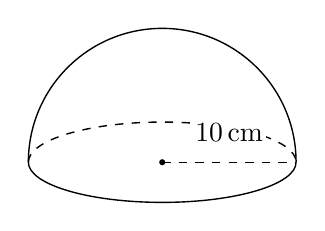
\begin{tikzpicture}[scale=0.85,line width=0.5pt]
  \draw (-2,0) arc (180:360:2 and 0.6);
  \draw[dashed] (-2,0) arc (180:0:2 and 0.6);
  \draw (-2,0) arc (180:0:2 and 2);
  \draw[dashed] (0,0) -- (2,0);
  \fill (0,0) circle (1.3pt);
  \node[fill=white,inner sep=1pt] at (1,0.45) {10\,cm};
\end{tikzpicture}

\par\vspace{4mm}
答(\underline{\hspace{32mm}})
\end{minipage}\hfill
\begin{minipage}[t]{0.48\textwidth}
(2)　次の円柱の表面積を求めなさい。\par\vspace{3mm}
\hspace*{4mm}
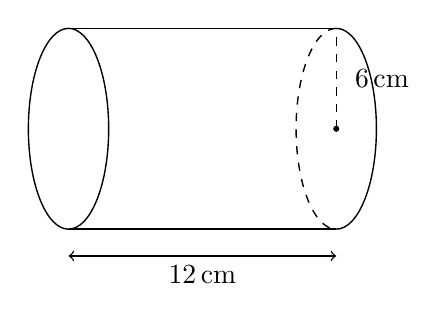
\begin{tikzpicture}[scale=0.85,line width=0.5pt]
  \draw (0,0) ellipse (0.6 and 1.5);
  \draw (0,1.5) -- (4,1.5);
  \draw (0,-1.5) -- (4,-1.5);
  \draw (4,-1.5) arc (-90:90:0.6 and 1.5);
  \draw[dashed] (4,1.5) arc (90:270:0.6 and 1.5);
  \fill (4,0) circle (1.3pt);
  \draw[dashed] (4,0) -- (4,1.5);
  \node[right=2pt] at (4.05,0.75) {6\,cm};
  \draw[<->] (0,-1.9) -- (4,-1.9);
  \node[below] at (2,-1.9) {12\,cm};
\end{tikzpicture}

\par\vspace{4mm}
答(\underline{\hspace{32mm}})
\end{minipage}

\end{document}
